\chapter{実装}
\label{implementation}

\section{Rive Client}
\subsection{システムフロー}

このシステムが立ち上がるとまず始めにonCreate()が呼ばれ、初期化を行う。
その後onStartInput()メソッドが呼ばれコンテキストを取得する。
このコンテキストはデバイスの情報を取得する。
コンテキストを取得し次第、候補単語を取得する。
この候補単語はサーバーと通信した上で取得する。
これをユーザーが一つの操作を行うたびに繰り返す。
ここで言う一つの動作とは、キーボード上の一つの文字を押すことや、
候補の単語をタップすること、
あるいは文字をデリートすることも含まれる。
最終的にユーザーが入力を終了した場合にはonFinishInput()が呼ばれ、
今回のユーザが行った動作とコンテキストを紐付けサーバーに送信する。
通信が終わり次第onDestory()が呼ばれ本システムは終了する。

\begin{figure}[htbp]
  \begin{center}
    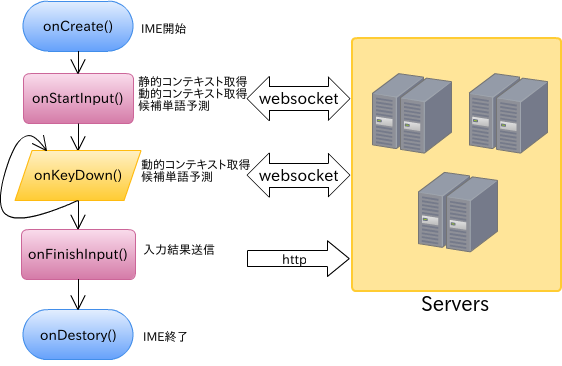
\includegraphics[width=12cm,bb=0 0 469 366]{images/clientflow}
  \end{center}
  \caption{Rive Clientフローイメージ}
  \label{fig:clientflow}
\end{figure}

\subsection{取得コンテキスト}
入力が開始されてから終了まで変わらないコンテキスト何度も取得すると
システムに負荷がかかるため、変わるものとそうでないものに分類した。
入力が開始してから変化しないコンテキストを静的コンテキスト。
入力が開始してから変化する可能性があるコンテキストを動的コンテキストとした。


\subsubsection{時間}
時間としてはunixtimeで4桁で取得
\subsubsection{位置情報}
\subsubsection{加速度}
\subsubsection{以前の入力}
\subsubsection{入力の状態}

\subsection{}

\section{Rive Server}

\section{Rive Analytics}

\section{Rive BatchProcessing}

\section{Rive WebService}
